\documentclass[a4paper,12pt]{article}

% Packages de base
\usepackage[utf8]{inputenc}
\usepackage[T1]{fontenc}
\usepackage[english,french]{babel}
\usepackage[margin=2.5cm]{geometry}

% Packages utiles
\usepackage{graphicx} % Pour les images
\usepackage{hyperref} % Liens cliquables
\usepackage{amsmath}  % Mathématiques avancées
\usepackage{enumitem} % Listes personnalisées
\usepackage{titling}  % Permet de mofif le title
\usepackage{float}    % Permet le positionnement des images

% Premiere page
\title{Python pour les incultes}
\author{Bodin Jules}
\date{\today}

\renewcommand{\maketitlehookd}{%
    \begin{center}
    
\includegraphics[keepaspectratio=true, width=0.8\textwidth]{../images/Logo_Python.jpg}
    \end{center}
}

\begin{document}

% Page de titre
\maketitle

% Page d'introduction avant la table des matieres
% Expliques comment est design ce pdf
\newpage

Ce document a pour but d'enseigner les rudiments de Python. Python est muni d'une multitude de packages\footnote{Un package en Python, 
c’est juste un dossier qui contient plusieurs fichiers Python (appelés modules) et qui permet d’organiser le code. 
} qui ne sont pas à connaitre dans le cadre d'une CPGE (cf. \href{https://prepas.org/ups.php?rubrique=53}{prepas.org}). 
Cependant, un de ces packages est très utile dans un cadre d'analyse de données : \textbf{matplotlib} et sera surement utilisé en physique. 
Je recommande donc de s'y intéresser et une page à la fin de ce cours y sera dédiée pour aborder les bases de ce package 
(il est très conséquent). \newline
\newline
Ce cours est construit pour être lu dans l'ordre des parties, mais il est aussi structuré pour permettre au lecteur de naviguer rapidement
et simplement dans ce dernier (car le temps c'est des places en prépa).
Il abordera toutes les notions nécessaires pour la prépa et plus encore, chaque point important étant accompagné d'un petit exemple. Attention cependant,
ces exemples ne suffiront pas à l'apprentissage de Python, seule la pratique régulière permettra de bien comprendre les notions abordées. \newline
\newline
Pour finir, le programme d'informatique pour tous aborde les notions de complexité des algorithmes étudiés. Ce cours donnera les complexités associées en les 
justifiant mais les preuves ne seront pas données, le but étant ici de comprendre la notion de complexité plus que de savoir la démontrer
(les profs seront bien meilleurs à ce niveau). \newline
\newline 
Je rappelle qu'aucune matière ne doit être négligée en prépa, cependant il est plus intéressant d'insister sur celles ayant un plus gros coefficient. 
Ainsi, il est plus intelligent de bien gérer son temps (encore lui) et de ne pas chercher à maitriser parfaitement ce cours durant les 2 années de prépa. 
Comme le disait si bien mon professeur de physique de permière année : la progression dans une matière est similaire à celle d'un circuit RC,
plus tu y passes de temps et moins l'évolution est grande (Je précise que c'est dans le cas d'une charge hein). \newline

\begin{figure}[H]
	\centering
	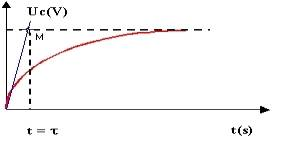
\includegraphics[keepaspectratio=true, width=0.8\textwidth]{../images/Charge_RC.jpg}
	\caption{Une charge de circuit RC au cas où le lecteur l'aurait oublié (pas bien ça)}
\end{figure}

\noindent Bonne lecture et bon courage, le chrono est déjà lancé.
\newpage

\tableofcontents % Table des matières optionnelle

\newpage

\section{Introduction}
Votre introduction ici.

\end{document}
